\documentclass[nobib, a4paper]{tufte-handout}

\title{Data-Driven Models for Zebrafish Motion}

\author[Lukas Krenz]{Lukas Krenz}

%\geometry{showframe} % display margins for debugging page layout
\usepackage{hyphenat}
\usepackage[
  style=verbose,
  autocite=footnote,
  backend=biber,
  doi=false,
  isbn=false,
  url=true
]{biblatex}
\addbibresource{../bibliography.bib}
% disable osf, https://tex.stackexchange.com/questions/56371/change-the-old-style-numerals-of-mathpazo-via-tufte-latex-to-lining-numerals?rq=1
\renewcommand{\rmdefault}{pplx} % todo remove later?

\usepackage{caption}
\usepackage{xpatch}
\usepackage{bm}
\usepackage{amsmath}
\usepackage{mathtools} % for \mathclap
\usepackage{varioref}
\usepackage{siunitx}
\sisetup{detect-all} % for correct fonts
\usepackage{placeins} % for \FloatBarrier
\usepackage{hyperref}
\usepackage[noabbrev]{cleveref}
\newcommand{\creflastconjunction}{, and\nobreakspace} % use Oxford comma
\usepackage{todonotes}
\usepackage{multimedia}
\usepackage{booktabs}
\newrobustcmd*{\bftabnum}{%
  \bfseries
  \sisetup{output-decimal-marker={\textmd{.}}}%
}
\usepackage{algorithm,algorithmicx}
\usepackage[noend]{algpseudocode}
\newcommand*\Let[2]{\State #1 \(\gets\) #2}
\algrenewcommand\algorithmicrequire{\textbf{Input: }}
\algrenewcommand\algorithmicensure{\textbf{Helper functions: }}

\usepackage{phaistos} % for fish symbol
\usepackage{tikz}
\usetikzlibrary{arrows, positioning, shapes.geometric}
\usetikzlibrary{calc}

\graphicspath{{../../figures/}}

% \usepackage{graphicx} % allow embedded images
%   \setkeys{Gin}{width=\linewidth,totalheight=\textheight,keepaspectratio}
%   \graphicspath{{graphics/}} % set of paths to search for images
% \usepackage{booktabs} % book-quality tables
% \usepackage{units}    % non-stacked fractions and better unit spacing
% \usepackage{multicol} % multiple column layout facilities
% \usepackage{fancyvrb} % extended verbatim environments
%   \fvset{fontsize=\normalsize}% default font size for fancy-verbatim environments

% Standardize command font styles and environments
\newcommand{\doccmd}[1]{\texttt{\textbackslash#1}}% command name -- adds backslash automatically
\newcommand{\docopt}[1]{\ensuremath{\langle}\textrm{\textit{#1}}\ensuremath{\rangle}}% optional command argument
\newcommand{\docarg}[1]{\textrm{\textit{#1}}}% (required) command argument
\newcommand{\docenv}[1]{\textsf{#1}}% environment name
\newcommand{\docpkg}[1]{\texttt{#1}}% package name
\newcommand{\doccls}[1]{\texttt{#1}}% document class name
\newcommand{\docclsopt}[1]{\texttt{#1}}% document class option name
\newenvironment{docspec}{\begin{quote}\noindent}{\end{quote}}% command specification environment

\begin{document}

\maketitle% this prints the handout title, author, and date

\begin{abstract}
\noindent
The goal of the project is to compare different data-driven models for the behavior of zebrafish.
The models should be able to predict and simulate the individual motion of an animal reacting to its environment.
The environment in our case is another fish and the walls surrounding the arena.
The models can be used to steer a fish in a virtual reality environment, for example.

We approximate the movement by a piece-wise linear model.
The wall forces are fit using a force-based model.

We present multiple models for the social behaviour, starting with a linear receptive field model.
This model is then enhanced by considering temporal dependencies and non-linear effects.
The final model is able to capture the entire trajectory distribution conditioned on the surroundings of the fish for each linear segment.
We achieve that using a mixture density recurrent neural network model.
\end{abstract}

\section{Introduction}
The goal of the project is to compare different strategies for modelling the behaviour of juvenile zebrafish.
These models should be able to predict and simulate the individual motion of one animal reacting to its environment (i.e.\ another fish and a wall).

A use-case for this project is steering a virtual fish in a virtual reality environment for animals.
It can be used to perform experiments that investigate causal relationships in animal behaviour.

The movement of zebrafish can be described by discrete models that assume that the fish moves in a piece-wise linear fashion.
After choosing a heading direction, the fish kicks off and moves in an approximately straight line.
We model the heading change and distance for each kick.

We start with an simple model and refine it twice.
Each modification drops assumptions about the behaviour and thus creates a more flexible, data-driven model.
The models developed in the earlier steps serve as baselines for the more complicated ones.
We can thus see whether the assumptions are correct and how important each component of the model is.

We make the following contributions:
\begin{itemize}
\item We discuss a force-based model for the wall--fish interaction.
\item We develop an data-driven receptive field approach for efficient spatial binning.
\item We evaluate whether including past receptive field improves the performance of the model.
  In other words, we evaluate whether the fish considers only its surroundings at kick-off time, or whether it posses a memory.
\item We present a recurrent neural network that can handle multi-modal predictions and captures non-linear effects.
  This model describes the trajectory distribution directly instead of performing only a point estimate.
\end{itemize}

\section{Pre-Processing}
Before we can dive into the modelling, we need to massage the data into an appropiate format.
This pre-processing stage is described in this chapter.
We first extract motion features from positions and orientations extracted by a video tracking software.
Then we segment the continous motion into discrete kicks.
All steps mentioned thus far follow the protocol of \citeauthor{calovi}\autocite{calovi} with slight modifications.
We then describe a simple wall model.
This model is considered a part of the pre-processing stage because we use it to filter the data to areas with weak wall influence.
We close this section with a description of our receptive field features that are a flexible representation of the surroundings of the animals.

\subsection{Experimental Setup \textit{\&} Input Data}
\begin{marginfigure}
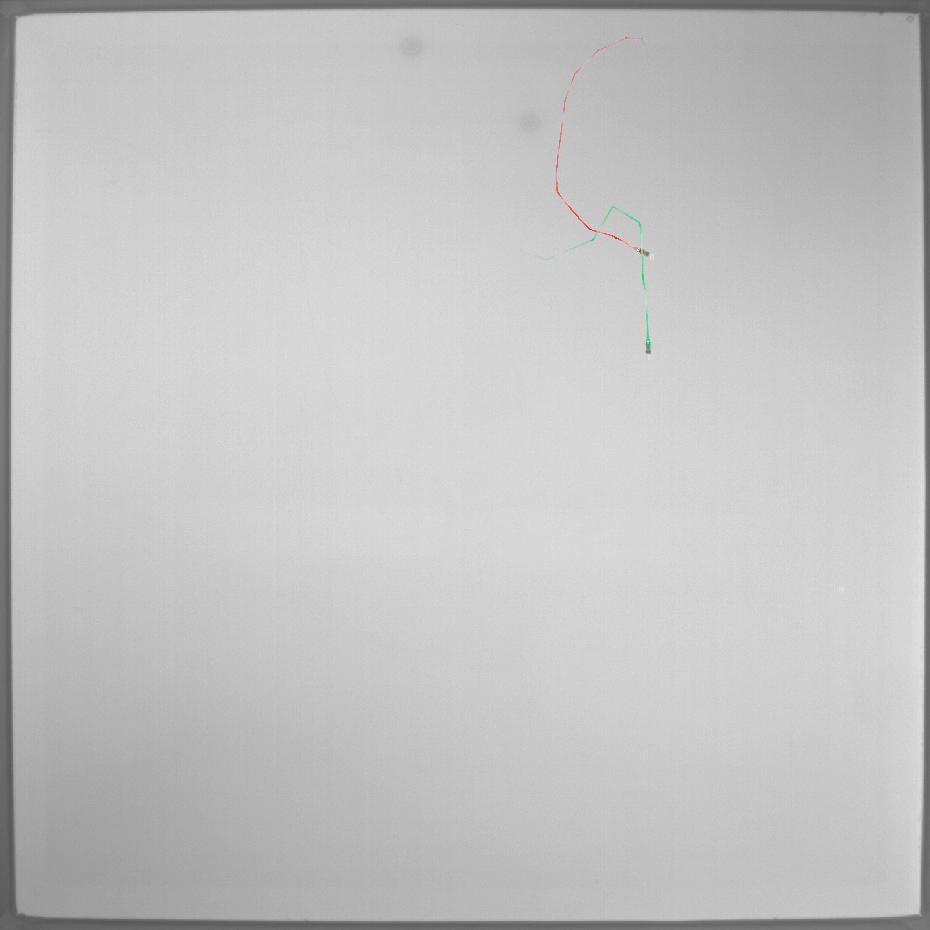
\includegraphics[width=\columnwidth]{tracked_frame}
\caption{Example frame of the tracked video.
  Shown is the \(\SI{30}{\cm} \times \SI{30}{\cm}\) large arena with two fish.
  The red and green lines show the fish trajectories that were estimated by the tracking software.
\label{fig:arena}}
\end{marginfigure}

We use data obtained from ten experiments.
In each experiment two fish swam for one hour in a \(\SI{30}{\m} \times \SI{30}{\m}\) tank, enclosed by a four straight walls.
The motion was captured by a camera and was tagged by a video tracking software.
An example for the experimental situation can be seen in figure~\ref{fig:arena}.
The raw data consists of the positions of both fish, their orientation relative to the x-axis, and time.

We mark frames that caused problems for the tracking system, for example when the identity of both fish was confused, as invalid.
The video data has roughly 100 frames per second, the time between frames is slightly irregular.
We convert the video to a constant framerate by iterating over the frames and insert frames between them if the time between frames differs by more than \SI{0.005}{\s} from a constant framerate.
These inserted frames are marked invalid as well.

The velocity is computed by finite differences between timepoints.
We then smooth the velocity by a Savgol filter with window length of 15 frames and a polynomial order of three.
This filter uses a local polynomial approximation, it is also used to compute the derivative of the velocity.
If fish move slower than \SI{0.5}{\cm/\s} for \SI{4}{\s}, they are marked as stopped.
Frames in that area are marked as invalid.
We do this because we are only interested in swimming behavior.

\subsection{Discrete Motion}
The movement of zebrafish can be described by discrete models that assume that the fish moves in a piece-wise linear fashion.
After choosing a heading direction, the fish kicks off and moves in an approximately straight line.
We need to segment the fish motion into kicks first.
Without loss of generality, we only consider how to segment the motion of one fish.
The segmentation for each fish is computed seperately, the resulting kicks are concatenated.

\begin{marginfigure}
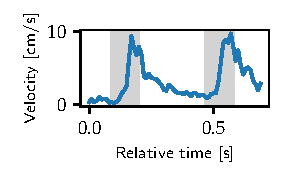
\includegraphics[scale=1]{smoothing}
\caption{Example result of the segmentation procedure.
  Shown is (non-smoothed) velocity.
  Areas shaded in gray were marked as acceleration, others as gliding.
\label{fig:smoothing}}
\end{marginfigure}

We then use the zero crossing of this smoothed acceleration to mark instances, where the fish moves from accelerating to gliding.
An example result for this method can be seen in figure~\ref{fig:smoothing}.
One acceleration and gliding phase is then combined to form a kick.
If an acceleration or gliding phase is shorter than a treshold \SI{0.08}{\s} the phase is merged with the previous one.
This segmentation procedure results in c.a.\ 148000 kicks.

We then extract the heading change, length, maximum velocity for each kick.
Additionally, we extract the positions and angles of both fish and the distance and angles towards the wall for both fish for the kick and timesteps before it.
For our experiments we use time steps of \SI{0}{\s}, \SI{0.05}{s}, \ldots, \SI{0.35}{\s}, which goes back roughly one mean kick duration (figure~\ref{fig:kick-duration}).
\begin{marginfigure}
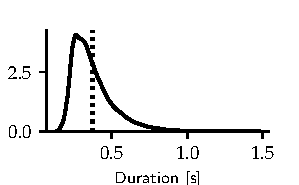
\includegraphics{kick_duration}
\caption{Kernel density estimate of training kick duration.
Dotted line is the mean duration at \SI{0.37}{\s}.}
\label{fig:kick-duration}
\end{marginfigure}


\begin{marginfigure}
    \centering
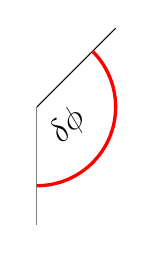
\begin{tikzpicture}[scale=0.5]
\draw[] (3, 3)--(5,5); % our fish at t
\node[rotate=45] at (4.5,4.5) {\textcolor{red}\PHtunny}; % head

\draw[gray] (3.0, 0)--(3.0, 3.0); % fish at t - 1
\node[rotate=90] at (3.0,2.5) {\textcolor{gray}\PHtunny}; % fish at t -1

\draw [red,very thick] (3.0, 1.0) arc (-90:45:2);
\node[rotate=45] at (3.8, 2.5) {\large$\delta\phi$};
\end{tikzpicture} 
\caption{Heading change from grey heading to red heading.}
\label{fig:goal}
\end{marginfigure}

This paper is concerned with the prediction of the relative change in orientation between the start and end of each kick (figure~\ref{fig:goal}).
The social models also predict the length of each kick.
We do not model the duration of the kicks, we rather draw them from a Gaussian mixture kernel density estimate fit to the experimental data.

\subsection{Wall Force}
We begin with the modeling of wall-forces.
We follow a force-based modeling approach and describe the influence of a wall on the heading change \(\delta \phi_w\) as
\begin{equation*}
  \delta \phi_w (r_w, \theta_w) = f(r_w)O_w(\theta_w),
\end{equation*}
where $r_w$ corresponds to the distance to the wall and $\theta_w$ is the relative angle of the fish towars the wall~\autocite{calovi}.
The relative angle is computed by subtracting the orientation of the fish from the orientation of the wall.
We split the wall influence into an exponentially decaying force term \(f_w\) and an odd angular-response function \(O_w\)
\begin{align*}
  f(r_w) &= \exp \left( -{(r_w/l_w)}^2 \right), \\
  O(\theta_w) &= c \left(a_1 \sin(\theta_w) + a_2 \sin(2  \theta_w)  \right)  \left(1 +  b_1  \cos(\theta_w) + b_2 \cos(2  \theta_w) \right),
\end{align*}
where $l_w, a_1, a_2, b_1, b_2 \text{ and } c$ are parameters.
Note that we use a different series expansion for the odd angular function \(O_w\).%
\footnote{Their proposed form does not work in our case.
  The reason for this could be that they consider both a different species and a round wall.}
Finally, we consider the closest two walls and sum over their influences
\begin{equation*}
 \delta \phi_w^{\text{total}} \left( \bm{r_w}, \bm{\theta_w} \right) = \sum_{\mathclap{i \in \, 2 \text{ closest walls}}} \delta \phi_w (r_w^i, \theta_w^i).
\end{equation*}

\begin{figure}[htb]
 \centering
 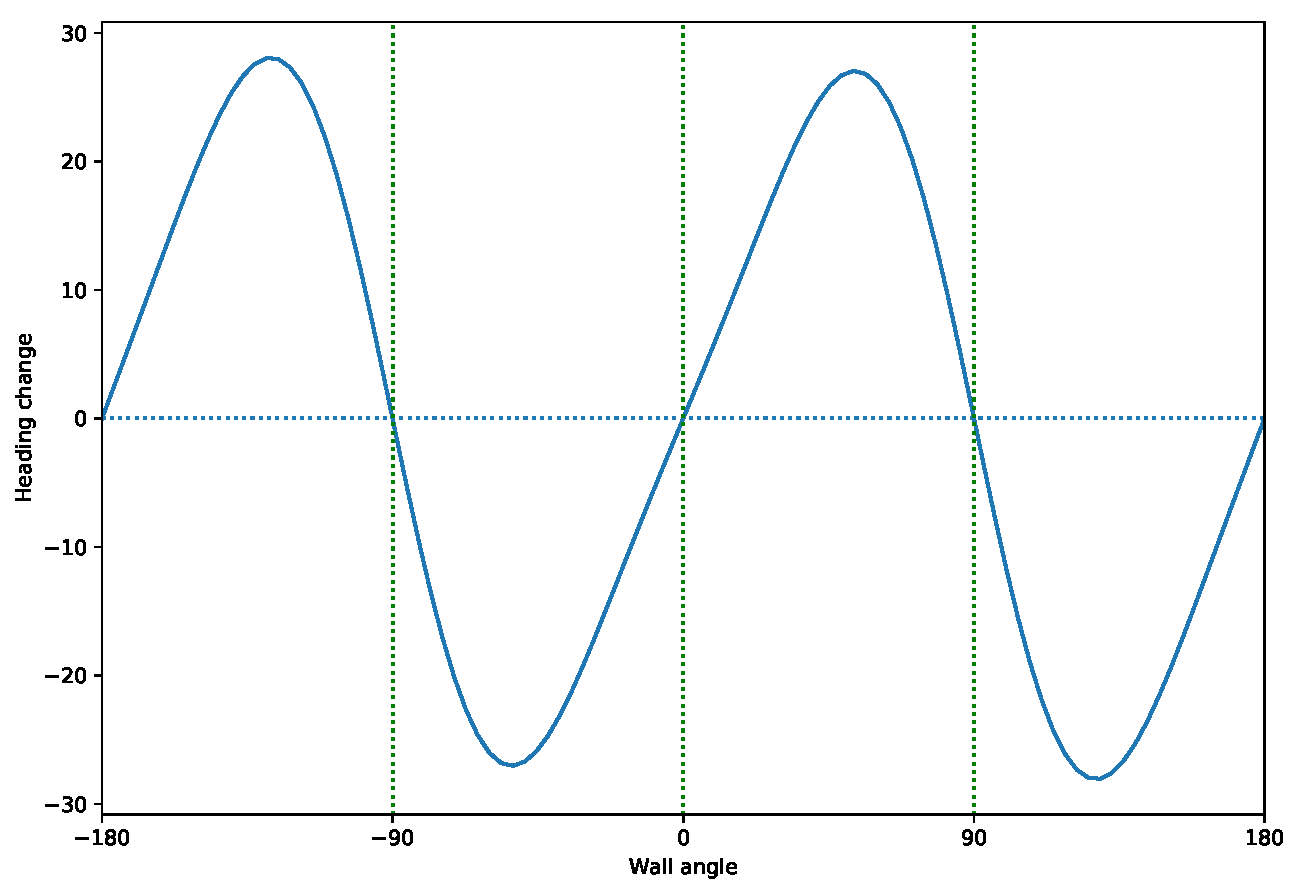
\includegraphics{wall_odd}~%
 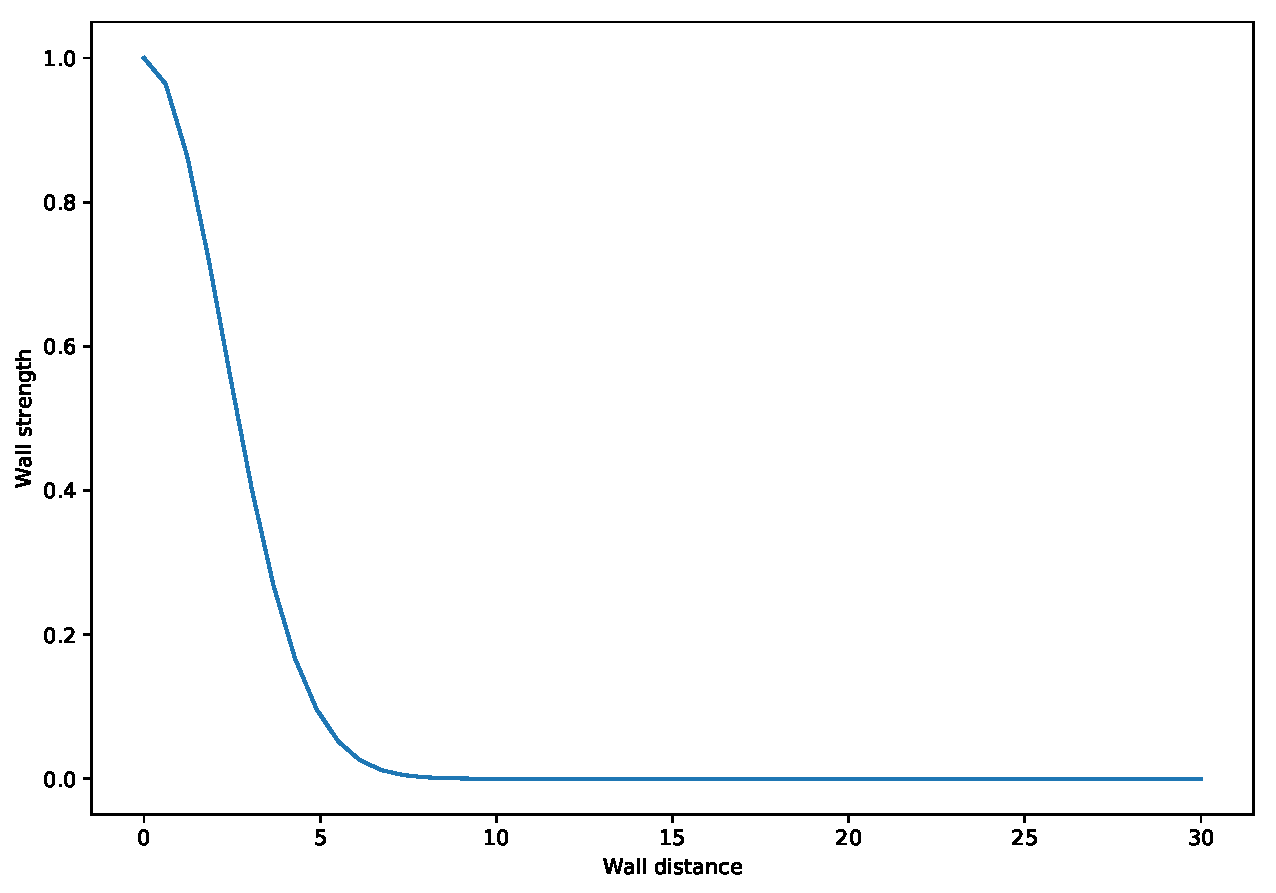
\includegraphics{wall_force} 
 \caption{Our wall fit.
   The force function is shown on the left, the exponentially decaying wall strength on the right.
 Positions of fixed points are shown by dotted lines.}
\label{fig:wall-fit}
\end{figure}

The parameters are fit by minimizing the mean-squared error of heading change prediction with the Levenberg-Marquardt algorithm using the implementation of \textbf{scipy}~\autocite{scipy}.
Our proposed functional forms result in a rapidly decaying wall influence (figure~\ref{fig:wall-fit}).

\subsection{Receptive Fields}
We now explain the input features of our social models.
From here on, we restrict our dataset to kicks where the wall influence is neglible.
Practically, we drop all kicks where the value of \(f_w(r_w)\) is larger than $0.1$.
This reduced the number of kicks in the training set to c.a.\ 19000.
Our social model use a receptive field as their input~\autocite{discreteModes}.
We construct this by rotating the coordinate system such that the fish we are considering is parallel to the x-axis and looking to the right.
This corresponds to a heading of \ang{0}.
We then shift the coordinate system such that our fish is at the center (figure~\ref{fig:rf}).

\begin{marginfigure}
 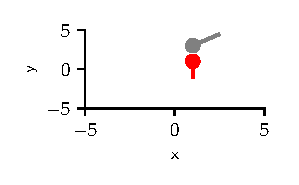
\includegraphics{receptive_field_before} 
 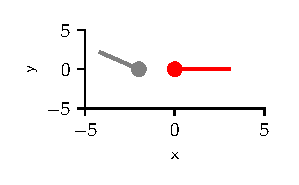
\includegraphics[scale=1]{receptive_field_after} 
 \caption{The receptive field transforms the situation depicted in the top figure to the one in the bottom figure.
 Note that the focal fish (red line) looks to the right which considered to be an orientation of zero in our coordinate system.}
\label{fig:rf}
\end{marginfigure}

Or models then try to predict the product of a vector in direction of the heading change and the kick length.
This correspond to the kick trajectory in our new coordinate system.

We now shift our focus to the spatial discretization.
The standard approach is to divide the space into a regular grid of bins with equal size.
This approach has the disadvantage that some bins contain most of the kicks while others are nearly empty.
One solution to lessen the impact of this problem is to introduce a cut-off range, after which the social forces are assumed to be neglible.
We do not follow this approach but rather use a data-driven binning approach where we try to create bins that have a more balanced occupancy.
This is not the only criterion for choosing a discretization approach.
For interpratibility it is useful to be able to clearly distinguish situations where the other fish is behind or in front of the focal fish and whether it is on its left or right side.
The algorithm to compute the bin edges is shown in algorithm~\ref{alg:binning}.
We only show how to compute the bins for the training set, the bins for the testing set can be computed in the same manner but without recomputing the edges.

Using a regular grid with 64 bins covering all seen positions (i.e.\ the minimum and maximum $x$ and $y$ coordinates are included in the grid) results in a mean number of fish per bin of roughly \(2077\pm 7255\) (mean $\pm$ std.) for the training set and \(474 \pm 1645\) for the testing set.
In fact, 12 and 13 of the bins actually do not contain any fish at all for the training and testing set respectively!
In contrast to that the bins of our proposed data-driven binning scheme contain $2077 \pm 179$ fish with zero empty bins for the testing scheme.
For the testing dataset the bins contain $474 \pm 139$ fish, again with zero empty bins (figure~\ref{fig:occupancy}).

\begin{figure}[htb]
  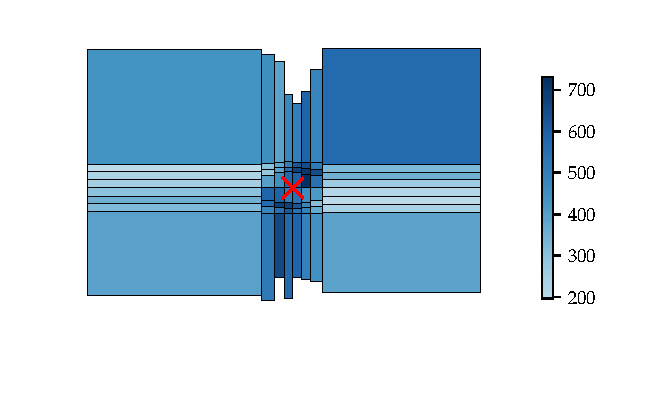
\includegraphics{rf_occupancy_test}
   \centering
   \caption{Number of fish in each bin obtained from data-driven binning scheme, evaluated on testing set.
     The color corresponds to the number of fish in per bin.
   The red cross marks the origin and thus the position of our focal fish.}
   \label{fig:occupancy}
\end{figure}

\MakeRobust{\Call} % allow stacking of call
\begin{algorithm}[htb]
  \caption{%
\label{alg:binning}
    Data-driven Spatial Binning}

  \begin{algorithmic}
    \Ensure{\\$\textsc{Edges} (\bm{x}, N)$ computes the edges of a histogram s.t.\ all $N$ bins have the same number of elements.
      If this is not possible, the first few bins have a size that is 1 larger.\\
    $\textsc{Bin} (\text{edges}, \bm{x})$ computes the histogram bin from the bin edges with open boundaries on both sides.}
   \Function{Edges-1d}{$\bm{x}$}
    \Let{$\text{edges}^-$}{\Call{Edges}{$\bm{x} [\bm{x} \leq 0]$}}
    \Let{$\text{edges}^+$}{\Call{Edges}{$\bm{x} [\bm{x} > 0]$}}
    \State \Return \Call{Concatenate}{$\text{edges}^-, 0, \text{edges}^+$}
\EndFunction 
\Require{Positions of focal fish $(\bm{x}, \bm{y})$ an number of bins per axis $N$}
\Let{bins}{\Call{Array}{size = \Call{Len}{$\bm{x}$}}}
\Let{edges-x}{\Call{Edges-1d}{$\bm{x}$}}
  \Comment{First bin x-axis}
  \Let{bins-x}{\Call{Bin}{edges-x, $\bm{x}$}}
  \Let{edges-y}{\Call{Array}{$\text{size} = N$}}
  \For{$\text{bin-x} \in \text{bins-x}$}
  \Comment{Bin y-axis for each x-bin seperately}
  \Let{idx}{$(\text{bins-x} = \text{bin})$}
  \Let{$\bm{y}^{\text{cur}}$}{$\bm{y} [\text{idx}]$}
  \Let{$\text{edges-y}[\text{bin-x}]$}{\Call{Edges-1D}{$\bm{y}^{\text{cur}}$}}
  \Let{$\text{bins}[\text{idx}]$}{$\text{bin-x} \cdot N + \text{edges-y}[\text{bin-x}]$}
\EndFor
\Return{edges-x, edges-y, bins}
\end{algorithmic}
\end{algorithm}

This categorical feature is converted using one-hot-encoding to a feature vector.
We additionally use the standarized relative trajectory of the other fish multiplied with the aforementioned spatial feature%
\marginnote{This can be generalized to multiple fish by interpreting the features as number of fish per bin and mean relative trajectory per bin.}.

\section{Social Models}\label{sec:social}
We are now ready to model the social behaviour of zebrafish.
Note that the approaches developed here can all be easily extended to larger fish groups.
Our target variable for all models is the relative kick trajectory in the local coordinate system described in the previous section.
We thus model heading change and distance jointly.%
\footnote{This approach has two advantages.
  Firstly, we avoid dealing with cyclic data (as angles are).
Secondly, all target variables (i.e.\ vector components) have the same phsyical dimension and unit which makes the loss functions easier to interpret.}
We start with a simple linear model.
This model is then refined twice by adding memory and non-linear effects.

\subsection{Linear receptive field model}
\begin{marginfigure}
  \begin{tikzpicture}[scale=0.5]
   \draw[ultra thick] (0,0)--(0,5);
   \node[rotate=45] at (4.5,4.5) {\textcolor{red}\PHtunny};
   \node[rotate=90] at (2.5,2.5) {\PHtunny};
   \node[rotate=90] at (2.5,0.5) {\textcolor{white}\PHtunny}; % quick hack to align stuff
 \end{tikzpicture}
 \caption{Situation considered for the models without memory:
 We model the heading change of the red fish given the current position and angle of the other fish.}
\end{marginfigure}

The linear model for a component \(i\) of our target vector \(\hat{\bm{y}}\) can be written as
\begin{equation*}
 \left( Y^i | \bm{\beta}^{i} \right)  \sim \mathcal{N} \left( \bm{X^i} \bm{\beta^i} + \text{ bias}, \sigma^2 \bm{I_{n \times p}}  \right),
\end{equation*}
where \(\bm{X^i}\) is the design matrix. \todo{mention weights, bias, identity matrix.}
In the following discussion of the linear models we will drop the superscript for the component and describe the computation for one vector component without loss of generality.

\subsection{Time dependence}
\begin{marginfigure}
  \begin{tikzpicture}[scale=0.5]
   \draw[red] (3, 3)--(5,5); % our fish
   \draw[ultra thick] (0,0)--(0,5); % wall
   \draw[gray] (2.5, 0)--(2.5,2.5);
   \node[rotate=45] at (4.5,4.5) {\textcolor{red}\PHtunny};
   \node[rotate=90] at (2.5,2.5) {\PHtunny};
   \node[rotate=90] at (2.5,0.5) {\textcolor{gray}\PHtunny};
 \end{tikzpicture}
 \caption{Situation considered for the models with memory:
   We model the heading change of the red fish given the trajectory of the other fish.
 The trajectory of the red fish is implicitely encoded in the receptive field as we consider the position of the other fish in the local coordinate system at each point of red's trajectory.}
\end{marginfigure}
We now add a time-dependence to our model.
To do this, we extract some time window before each kick.

We consider two more models here.
For the first one we simply concatenate all features of the design matrix \(\bm{X_t}\) for all timesteps \(t\).
This results in a very large number of parameters, consisting of one set of weights \(\bm{\beta_t}\) per timestep.

Alternatively, we can use the same spatial weights for each timestep (i.e\ \( \forall t_1, t_2: \bm{\beta_{t_1}} = \bm{\beta_{t_2}}\)).
We introduce a parameter \(c_t\) with one weight per timestep and then use $c_t \bm{\beta}$ as our parameters.
For consistency, we normalize all \(c_t\) such that they are positive and sum to unity using the \textit{softmax} non-linearity
\begin{equation}\label{eq:softmax}
\operatorname{Softmax} (x_i) = \frac{\exp (x_i)}{\sum_j \exp (x_j)},
\end{equation}
where \(x_i\) is one component of the output vector.

The prediction is then given by
\begin{equation*}
  \hat{y} = \sum_t c_t \bm{X_t} \bm{\beta} + \text{ bias}.
\end{equation*}

\subsection{Mixture Density Networks: Bi-modal distributions \textit{\&} non-linearity}
As a final model we present a recurrent-neural network that predicts a full distribution for \(\left( \bm{y} | \bm{\beta} \right)\).
We start by describing an encoder, which transforms the input features to a hidden state, and a decoder which then transforms the hidden state into the output values.
The complete model is then an arbitrary combination of presented encoders and decoders.

We describe two simple encoders:
\begin{itemize}
\item The simplest (non-linear) choice is a multilayer-perceptron (\textsc{mlp}).
  In our case we use a two layers consisting of a linear transformation, followed by the \textit{tanh} non-linearity and a dropout probability of 50\%\autocite{dropout}.
  The input features for this model is the receptive field for the kick-off time.
\item
  As a temporal model we consider a standard recurrent neural network (\textsc{rnn}) which has an input linear transformation, and a recurrent hidden-to-hidden connection.
  For the hidden-to-hidden connection we apply recurrent dropout\autocite{recurrentDropout}.
  This means that we sample a dropout mask per example and apply this to the hidden-to-hidden connections for all sequence steps instead of sampling a seperate mask for each sequence step.
  We denote this dropout operator as \(d(\bm{x})\).
  These two layers are added and transformed with a \textit{tanh} non-linearity
  \begin{equation*}
    \bm{h^i} (\bm{x}) = \operatorname{tanh} \left( \bm{b} + \bm{w_{ih}} \bm{x^i} + \bm{w_{hh}} d (\bm{h^{i-1}}) \right),
  \end{equation*}
  where \(\bm{w_{ih}}\) and \(\bm{w_hh}\) are the weights for the input-to-hidden and hidden-to-hidden layers respectively.
  The parameter \(\bm{b}\) corresponds to a vector of learned biases.
  We learn the initial hidden state \(h^0\) instead of using a zero-initialised state as it improved the speed of convergence.

  The input features for this models is the complete sequence of receptive fields leading to a kick.
  We use a fixed input sequence length for two reasons:
  Firstly, this allows us to compare the time-dependent linear models and \textsc{rnn}-models directly.
  Secondly, we avoid the assumption that a fish only considers its surroundings in the timespan between two kicks.
  Note that we have assume that a kick is independent of the other kicks.
\end{itemize}
We did not observe significant better results using the rectifier linear unit activation function, in fact, it lead to divergence for the \textsc{rnn} model.
Using more neurons in the hidden layer does not achieve better results here.
For scenarios with less sparse feature vectors such as with larger fish groups, a more complex representation might be beneficial.
We hope that the combination of the simplicity of the models coupled with the dropout regularization leads to a highly representative compressed representations in the encoded vector.
Note that both models (disregarding the learning initial \textsc{rnn}-state) have the same number of parameters.

For the encoder we follow the ideas of \textit{mixture density networks} but use multivariate Gaussians with non-diagonal covariance as mixture components\autocite{mdn}.
To do this, we write our prediction as
\begin{equation*}
p \left( \bm{y} | \bm{\beta} \right) = \sum_{i}^n \pi_i \mathcal{N} \left( \bm{\mu_i}, \bm{\Sigma_i} \right),
\end{equation*}
where \(\pi_i, \bm{\mu_i}, \bm{\Sigma_i}\) are the parameters (mixing coefficients, mean and covariance) for a mixture of Gaussians with \(k\) components.
The function \(\mathcal{N}(\bm{\mu}, \bm{\Sigma_i})\) is the probability density of a multivariate normal distribution 

These parameters are predicted for each target seperately by our neural network.
We will now derive necessary conditions that have to hold for the parameters and describe how our network output satisfies them.
Note that we can write the Cholesky decomposition%
\footnote{This decomposition always exists for invertible covariance matrices as they are by definition positive-semidefinite and symmetric.}
of the covariance matrix \(\bm{\Sigma_i}\) as
\begin{equation*}
  \bm{\Sigma_i} = \bm{L_i} \bm{L_i^T} =
  \begin{bmatrix}
    a_i^2 & a_ib_i \\
    a_ib_i & b_i^2 + c_i^2
  \end{bmatrix} ,\quad
   \text{with } \bm{L} =
   \begin{bmatrix}
     a_i & 0 \\
     b_i & c_i
   \end{bmatrix}.
\end{equation*}
We then have to fulfil the following constraints:
\begin{itemize}
\item The diagonals of all \(\bm{L}_i\) need to be larger than zero.
  To do this we use the \textit{exponential function} as our non-linearity
  We add a small \(\varepsilon = \sqrt{10^{-6}}\) for numerical stability%
  \footnote{This regularization reduces the condition number of \(\bm{\Sigma_i}\) by increasing the value of its minimal eigenvalue.
  Additionally it ensures that the variance has a minimal value and thus avoids degenerate distributions.}. % maybe cite this master's thesis?
  Using the fact that a matrix has an invertible Cholesky decomposition with positive diagonal elements iff.\ it is positive definite and Hermetian,
  the resulting matrix \(\bm{\Sigma_i}\) is a valid non-singular covariance matrix.
\item The mixing coefficients need to be positive and have to sum to one.
  This is achieved by using the \textit{softmax} (equation~\ref{eq:softmax}) non-linearity.

\end{itemize}
All other parameters can have arbitrary values.
We predict the Gaussian mixture parameters each by computing a linear transformation of the hidden state of the encoder followed by the appropiate non-linearity.
Using a full covariance matrix instead of a diagonal lead to no improvement for our data.
Because a diagonal covariance matrix is conceptually simpler, we set \(b_i\) to zero for all outputs.%
\sidenote{This does not limit the capabilities of our network because a mixture of Gaussians with diagonal covariance matrices is able to approximate all non-degenerate distributions,
  given a sufficient number of components.}

We minimize the negative-log-likelihood, which is given for a vector of examples \(\bm{y}\) by
\begin{align}
  \label{eq:nll}
 \mathcal{L} (\bm{y}; \bm{\pi}, \bm{\Sigma}, \bm{\mu}) &= - \log \left(  \sum_i \exp \left(  \log \left( \bm{\pi_i} \mathcal{N} (\bm{y}; \bm{\mu_i}, \bm{\Sigma_i} \right) \right) \right) \\ 
  \intertext{with}
  \log \left( \mathcal{N} (\bm{y}; \bm{\mu_i}, \bm{\Sigma_i}) \right) &= 
 -\log \left( \sqrt{\pi_i^2 \vert \bm{\Sigma_i}} \vert)  \right) - 0.5 \left( (\bm{y} - \bm{\mu_i})^T \bm{\Sigma_i}^{-1} (\bm{y} - \bm{\mu_i}) \right),\nonumber
\end{align}
to train our models.
In this equation, \(\vert \bm{\Sigma_i} \vert\) denotes the determinant of \(\bm{\Sigma_i}\)%
\sidenote[][-1cm]{We compute the determinant directly from the Cholesky matrix \(\bm{L_i}\).
  Furthermore we do not invert the covariance matrix but rather solve the equivalent linear system with forward-backward substitution using \(\bm{L_i}\) again.
For the diagonal case, both determinant and inverse are trivial to compute and numerically stable.}.
While this optimization problem is mathematically correct, it is suspectible to underflow.
To rectify this we follow common advice and apply the \textit{log-sum-exp-trick} which is given by the identity
\begin{equation*}
  \log \left( \sum_i \exp (x_i) \right) = \max_i (x_i) + \log \left( \sum_i \exp (x_i - \max_i (x_i)) \right)
\end{equation*}
to compute the sum in equation~\ref{eq:nll}\autocite{mdnMaster}.

\section{Implementation \textit{\&} Training Details}
The linear model without memory and the one with concatenated features were trained with the \textit{RidgeCV} estimator from \textbf{scikit-learn}\autocite{scikitLearn}.
This implementation uses generalized-cross-validation over the training set to determine the best parameter for the regularization strength.

%The linear model with identical spatial weights was implemented in \textbf{PyTorch} and optimized with the \textsc{L-BGFS} optimizer until convergence~\autocite{pytorch}.
The linear model with static spatial weights and all neural network models were implemented in \textbf{PyTorch}.
The number of components for the \textsc{mdn}-networks was is set to 5.
We use stochastic gradient descent with an initial learning rate of 0.1 and a weight decay of 0.0001 to optimize our networks.
We apply a Nesterov momentum of 0.9.
Encoders and decoders are jointly trained.
We clip gradients such that they have a maximum absolute value of 100 for stability of training.
For initialization, weights are drawn from a normal distribution with mean 0 and standard deviation of 0.002 and all biases are set to zero.
We train all models for 1000 epochs with a batch size of 128.

We implemented a program to output an animation that shows two fish swimming, each controlled by one of our implemented algorithm.
The simulation uses periodic boundary condition to show the effect of the social models without the influence of walls.

A possible use case for these models is steering a virtual fish in a virtual reality environment.\todo{cite fish vr, does it belong here?}
In this case periodic boundary conditions are possible but are not meaningful.
To rectify this, one can predict the heading change with our social models and then rotate the resulting trajectory by the prediction of the wall model.
Alternatively it would be possible to implement a virtual force that pushes our fish away from the wall.
This is of course not physical but would allow us to observe the social behaviour.

\section{Evaluation}
\begin{margintable}[5cm]
\centering
\begin{tabular}{@{}lS[table-format=1.3]S[table-format=1.3]@{}}
\toprule
{Model} & {Angle-Train} & {Error-Test} \\ \midrule
Mean & 0.398 & 0.375 \\ 
  Calovi & \bftabnum 0.379 & \bftabnum 0.350\\ %should not need linebreak here
\bottomrule\\
\end{tabular}
\caption{Results for angular model.
  Angle-\{Train/Test\} refers to equation~\ref{eq:angle-error}.
  Best results are bold.
}
\label{tab:results-wall}
\end{margintable}

We start by comparing the angle prediction from the wall model against the baseline of always predicting the mean angle.
Evaluating these predictions with the mean-squared-error (\textsc{mse}) or similar metrics is not meaningful because they do not take the cyclical nature of angles into account.
For example, a prediction of \ang{360} for an angle of \ang{0} would be perfect but would incur a large \textsc{mse}-loss.
We rectify this by using definitions from directional statistics\autocite{circularStatistics}.
% Angle error, https://stats.stackexchange.com/questions/197639/calculating-goodness-of-fit-for-circular-data
We can compute the mean of a vector of angles \(\bm{\alpha}\) with
\begin{equation*}
 \operatorname{Mean-Angle}(\bm{\alpha}) = \operatorname{arctan2} \left( \sum_i \sin \left( \alpha_i \right),  \sum_i \cos \left( \alpha_i \right)  \right).
\end{equation*}
One possible way of defining an error over angles is
\begin{equation}\label{eq:angle-error}
 \operatorname{Angle-Error}(\bm{\alpha}, \bm{\beta}) = \operatorname{Mean} \left( \operatorname{arccos} \left(  \cos  (\bm{\alpha} - \bm{\beta})  \right) \right).
\end{equation}
This error is zero if both angles are identical.
Our wall model achieves a lower error than predicting the mean for all examples on both training and testing data (table~\ref{tab:results-wall}).

We compare the models by the log-likelihood on the training and testing set.
Even though the linear models are not trained by optimizing the \textsc{nll}, it is appropiate to use this metric for evaluation.
The reason for this is that the regularized \textsc{mse} loss function used for ridge regression can be derived by computing the \textsc{nll} under the assumption that the likelihood is Gaussian plus a Gaussian prior on the weights.
As mentioned in section~\ref{sec:social}, both datasets are restricted to situations with neglible wall-force.
This comparison captures the whole predictive distribution and not only the mean prediction.
In this way we take the uncertainty of the predictions into account.
Note that it is not straight-forward to use more complicated methods such as log-likelihood ratios or the Akaike information criterion because we cannot estimate the number of degrees of freedoms for penalized recurrent neural network models.

The best \textsc{nll}-error was achieved by the \textsc{mlp-mdn} and \textsc{rnn-mlp} on the training and testing set respectively (table~\ref{tab:results-social}).
Interestingly, both methods have the best \textsc{mse}, even though we include models that were explicitely trained on the \textsc{mse}.
The linear models all had larger errors for all considered metrics but did not perform significantly worse.

\begin{table}[htb]
\centering
\caption{Results for all social models on training and testing datasets.
  Linear models are linear without time, linear with entire sequence concatened as features, linear with static spatial weights.
  Best results are bold.
}

\label{tab:results-social}
\begin{tabular}{@{}lS[table-format=1.2]S[table-format=1.2]S[table-format=1.3]S[table-format=1.3]@{}}
\toprule
{Model} & {\textsc{nll}-train} & {\textsc{nll}-test} & {\textsc{Mse}-train} & {\textsc{Mse}-test} \\ \midrule
Linear (w/o time) & 2.08 & 1.90 & 0.472 & 0.388 \\
Linear (time conc.) & 2.06 & $\infty$ & 0.459 & 0.385 \\
Linear (const.\ spatial) & 2.08 & 1.91 & 0.467 & 0.391 \\
\textsc{Mlp-Mdn} & 1.71 & \bftabnum 1.63 & 0.464 & \bftabnum 0.384 \\
\textsc{Rnn-Mdn} & \bftabnum 1.61 & 1.71 & \bftabnum 0.454 & \bftabnum 0.384 \\
\textsc{Mlp-Mse} & 2.08 & 1.90 & 0.468 & 0.388 \\
\textsc{Rnn-Mse} & 2.04 & $\infty$ & 0.449 & 0.392 \\
\bottomrule\\
\end{tabular}
\end{table}


\section{Conclusion \textit{\&} Future Work}
In this work we presented a full modelling pipeline for discrete social models with temporal and non-linear effects.
This pipeline starts by massaging the data into an appropiate format, using a wall model to filter timesteps with a strong wall influence, setting up a data-driven spatially discrete receptive field and finished with complex models implemented with a state-of-the-art neural network framework. 

Even though extending the models with a temporal and non-linear component did not show significant improvements for our dataset, we think that our proposed models are promising:
\begin{itemize}
\item The data-driven spatial discretization results in a more equal distribution of fish than a standard regular grid.
\item Because the social models do not use properties of other animals directly but rather model the mean features per bin they extend trivially to larger animal groups, without changing the statistical models or the spatial discretization.
  This extension is harder for force-based models and usually require extensive modifications of the core model.
  We believe that our models perform better for larger animal groups as this would result in less sparse input vectors.
\item The explicit modelling of probability distributions allows us to sample from the trajectory distribution conditioned on the social surroundings and is able to predict bimodal distributions.
\end{itemize}
These results can be used directly for large-scale moddeling of fish-swarms.
We recommend the collection of more data or increasing the data-efficiency of the models.
This could be achieved by
\begin{itemize}
\item Running more or longer experiments.
\item Lessening the impact of the restriction to areas with neglible wall influnce.
  This could be accomplished by using fish that do not swim close to the wall at most times, using different arenas or by using a model that incorporates both wall and social influences directly.
  The latter approach could also consider non-linear interactions between both kind of environmental forces.
\item Using a continous model instead of performing a segmentation into kicks.
  This could be problematic for juvenile zebrafish as naive \textsc{rnn} models might not be suited for the moddeling of different states of motion.
\end{itemize}

\printbibliography
\end{document}